
\documentclass{article}
\renewcommand{\labelenumi}{\alph{enumi}.}
\usepackage{amsmath}
\usepackage{amscd}
\usepackage[tableposition=top]{caption}
\usepackage{ifthen}
\usepackage[utf8]{inputenc}
\usepackage[pdftex]{graphicx}

\usepackage{Sweave}
\begin{document}
\title{Test 2}
\author{Christopher Peters}
\maketitle

{\bf This Exam is Individual Work. No Collaboration is Allowed}\\
\section{(15 points).}
Consider the probability paper given in Figure 1. Do the following:\\

\begin{figure}
  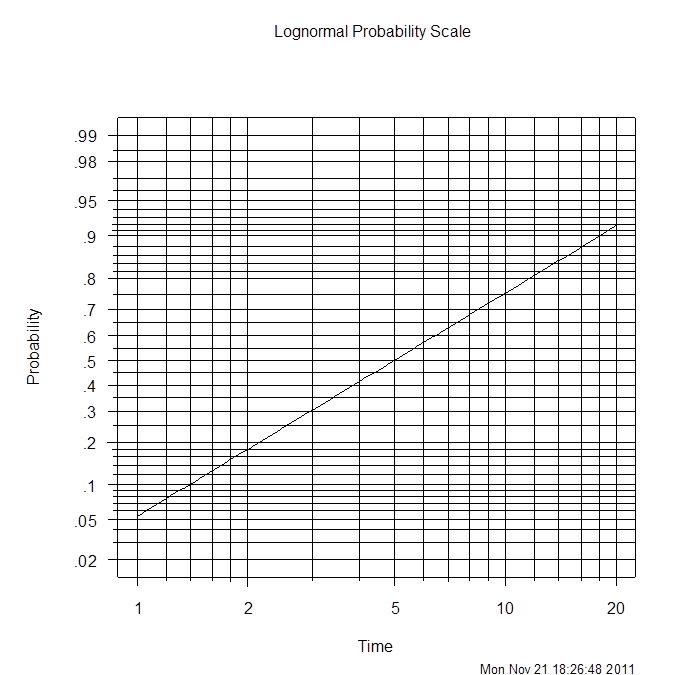
\includegraphics[width = 5in]{lognormal_graph_1.png}
  \caption{Lognormal Probability Plot}
\end{figure}

\subsubsection{} 
Plot on the paper the LOGNOR(exp( \mu ) = 5, \sigma = 1).



\end{document}
